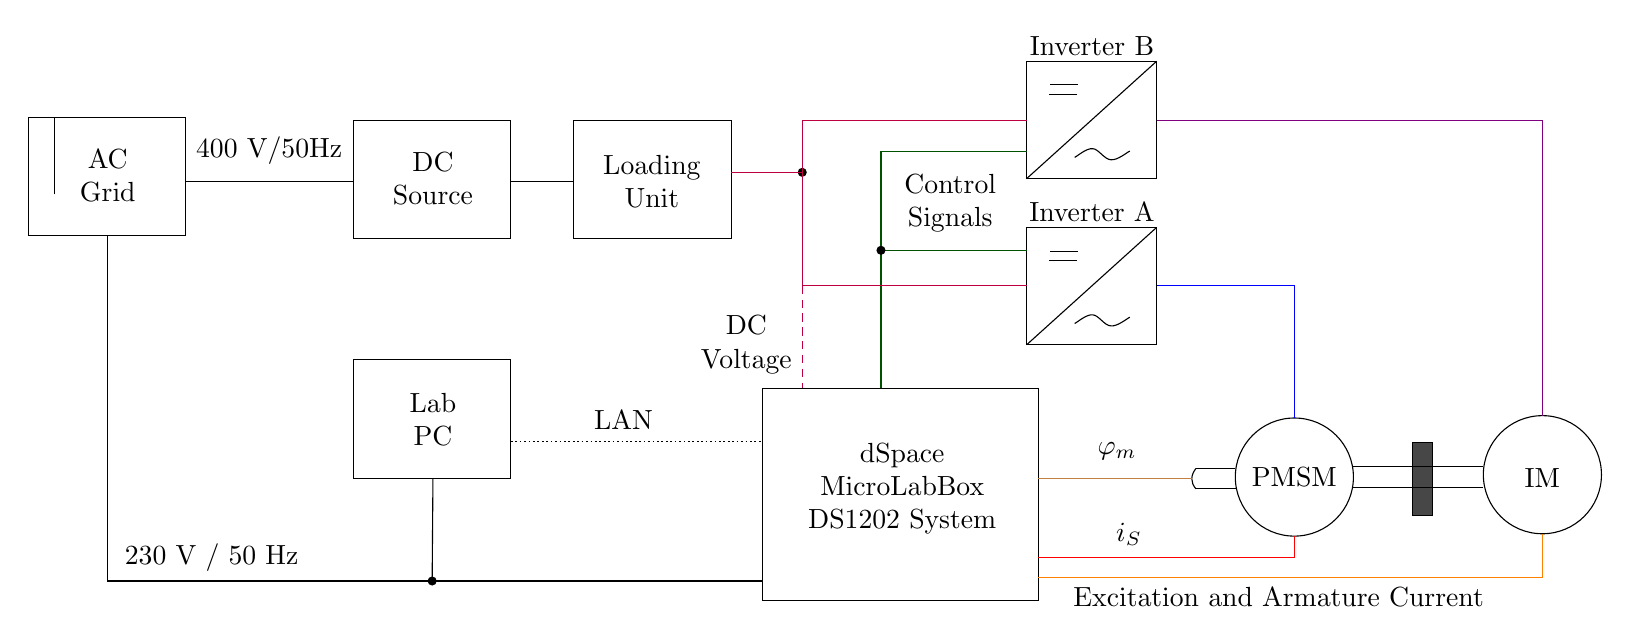
\begin{tikzpicture}
  \draw (-1.4,2.55) rectangle (0.6,1.05);
  \node[align=center] at (2.77,-2.13) {dSpace \\ MicroLabBox\\DS1202 System};
  \draw (-4.2,2.55) rectangle (-2.2,1.05);
  \node[align=center] at (-3.19,1.81) {DC \\ Source};
  \node[align=center] at (-5.27,2.16) {400 V/50Hz};
  \draw (-8.33,2.59) rectangle (-6.33,1.09);
  \node[align=center] at (-7.32,1.85) {AC \\ Grid};
  \draw (-8.33,2.59) grid (-8.33,1.61);
  \draw (-4.2,-0.49) rectangle (-2.2,-2);
  \node[align=center] at (-3.19,-1.25) {Lab \\ PC};
  \draw (1,-0.85) rectangle (4.5,-3.55);
  \draw (4.35,3.3) rectangle (6,1.81);
  \draw (4.35,1.81) -- (6,3.3);
  \draw (4.96,2.08) .. controls (5,2.1) and (5.11,2.2) .. (5.19,2.19) .. controls (5.26,2.19) and (5.34,2.05) .. (5.42,2.05) .. controls (5.5,2.04) and (5.62,2.14) .. (5.66,2.16);
  \draw (4.65,3) -- (5,3);
  \draw (4.64,2.88) -- (4.99,2.88);
  \node[align=center] at (5.18,3.49) {Inverter B};
  \draw (4.35,1.19) rectangle (6,-0.3);
  \draw (4.35,-0.3) -- (6,1.19);
  \draw (4.96,-0.03) .. controls (5,-0.01) and (5.11,0.09) .. (5.19,0.08) .. controls (5.26,0.08) and (5.34,-0.06) .. (5.42,-0.06) .. controls (5.5,-0.07) and (5.62,0.03) .. (5.66,0.05);
  \draw (4.65,0.89) -- (5,0.89);
  \draw (4.64,0.77) -- (4.99,0.77);
  \node[align=center] at (5.18,1.38) {Inverter A};
  \draw (10.9,-1.95) circle (0.75cm);
  \node[align=center] at (10.9,-1.99) {IM};
  \draw (7.75,-1.98) circle (0.75cm);
  \node[align=center] (node1) at (7.75,-1.98) {PMSM};
  \draw[fill=black!72] (9.25,-1.54) rectangle (9.5,-2.47);
  \draw (8.5,-1.85) -- (10.15,-1.85);
  \draw (8.49,-2.11) -- (10.15,-2.11);
  \node[align=center] at (-0.41,1.77) {Loading \\ Unit};
  \draw (7,-1.87) -- (6.5,-1.87);
  \draw (7.01,-2.13) -- (6.5,-2.13);
  \draw (6.5,-1.87) .. controls (6.43,-1.96) and (6.43,-2.05) .. (6.5,-2.13);
  \draw[brown] (6.45,-2) -- (4.5,-2);
  \node[align=center, minimum width=59pt] at (5.5,-1.65) {$\varphi_m$};
  \draw[red] (4.5,-3) -- (7.75,-3) -- (7.75,-2.73);
  \draw[orange] (10.9,-2.7) -- (10.9,-3.26) -- (4.5,-3.26);
  \node[align=center, minimum width=59pt] at (5.65,-2.71) {$i_S$};
  \node[align=center, minimum width=59pt] at (7.55,-3.5) {Excitation and Armature Current};
  \draw[blue] (6,0.45) -- (7.75,0.45) -- (7.75,-1.23);
  \draw[violet] (6,2.55) -- (10.9,2.55) -- (10.9,-1.2);
  \draw[green!32!black] (4.35,2.16) -- (2.5,2.16) -- (2.5,-0.85) -- (2.5,0.9) -- (4.35,0.9);
  \node[align=center] at (3.38,1.5) {Control \\Signals};
  \draw[fill=black] (2.5,0.9) circle (0.05cm);
  \draw[fill=black] (1.5,1.89) circle (0.05cm);
  \draw[purple] (0.6,1.89) -- (1.5,1.89) -- (1.5,2.55) -- (4.35,2.55);
  \draw[purple] (1.5,1.94) -- (1.5,0.45) -- (4.35,0.45);
  \node[align=center] (node2) at (0.79,-0.3) {DC \\ Voltage};
  \draw[densely dashed, purple] (1.5,0.45) -- (1.5,-0.85);
  \draw (-6.33,1.77) -- (-4.2,1.77);
  \draw (-2.2,1.77) -- (-1.4,1.77);

  \draw[densely dotted, semithick] (-2.2,-1.53) -- (1,-1.53);

  \node[align=center] at (-0.77,-1.26) {LAN};

  \draw (1,-3.3) -- (-7.32,-3.3) -- (-7.32,1.09);

  \node[align=center] at (-6,-3) {230 V / 50 Hz};
  \draw (-3.19,-2) -- (-3.2,-3.3);

  \draw[fill=black] (-3.2,-3.3) circle (0.05cm);
\end{tikzpicture}